\section{Serielle Datenübertragung - UART / I2C}
\subsection{UART - Universal Asynchronous Receiver Transmitter}
\begin{itemize}
    \item Benötigt Synchronisation am Anfang von jedem Daten-Frame
    \item Symbolrate = Bitrate (Baudrate = Bits pro Sekunde)
    \item 5-8 Datenbits, 1-2 Stopbits, 1 Startbit
    \item Parity-Bit: none, mark (1), space (0), odd, even
    \item Bei ungleicher Taktung: Asynchroner Modus
    \begin{itemize}
        \item Benötigt Overhead für Start- und Stopbits
    \end{itemize}
    \item Vorteil: CLK nicht notwendig, Übertragungslatenz wird kompensiert
\end{itemize}
\subsubsection{Implementierung eines UART-Transmitters}
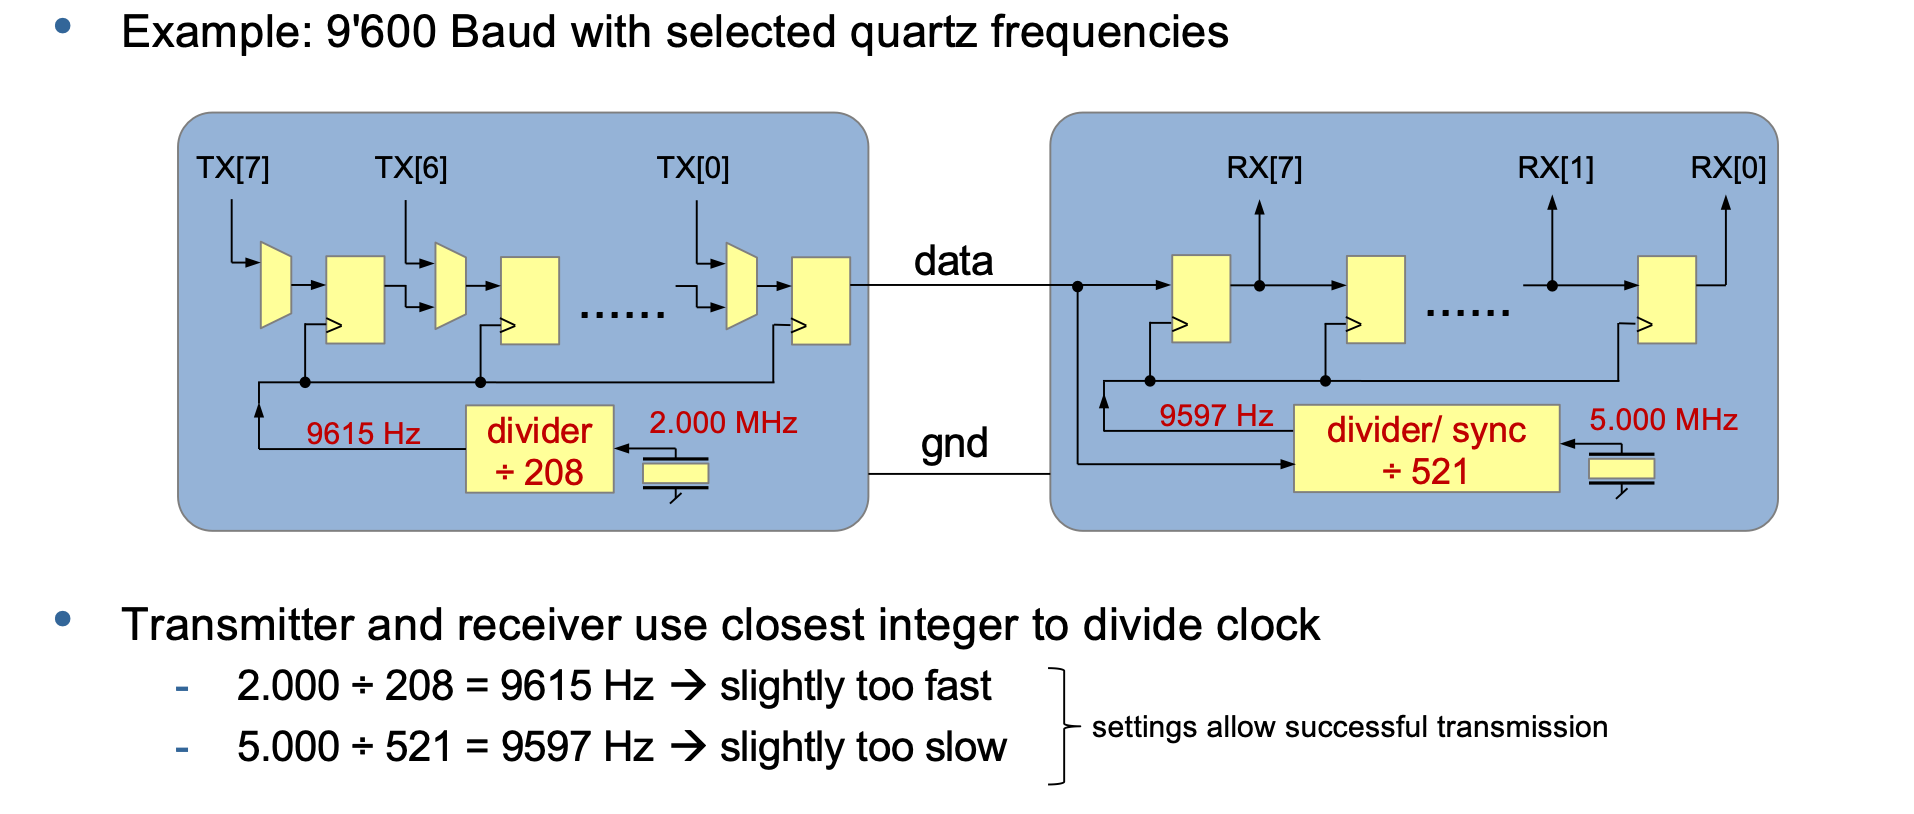
\includegraphics[width=0.3\textwidth]{sections/images/uart_impl.png}

\subsubsection{UART Timing Diagramm}
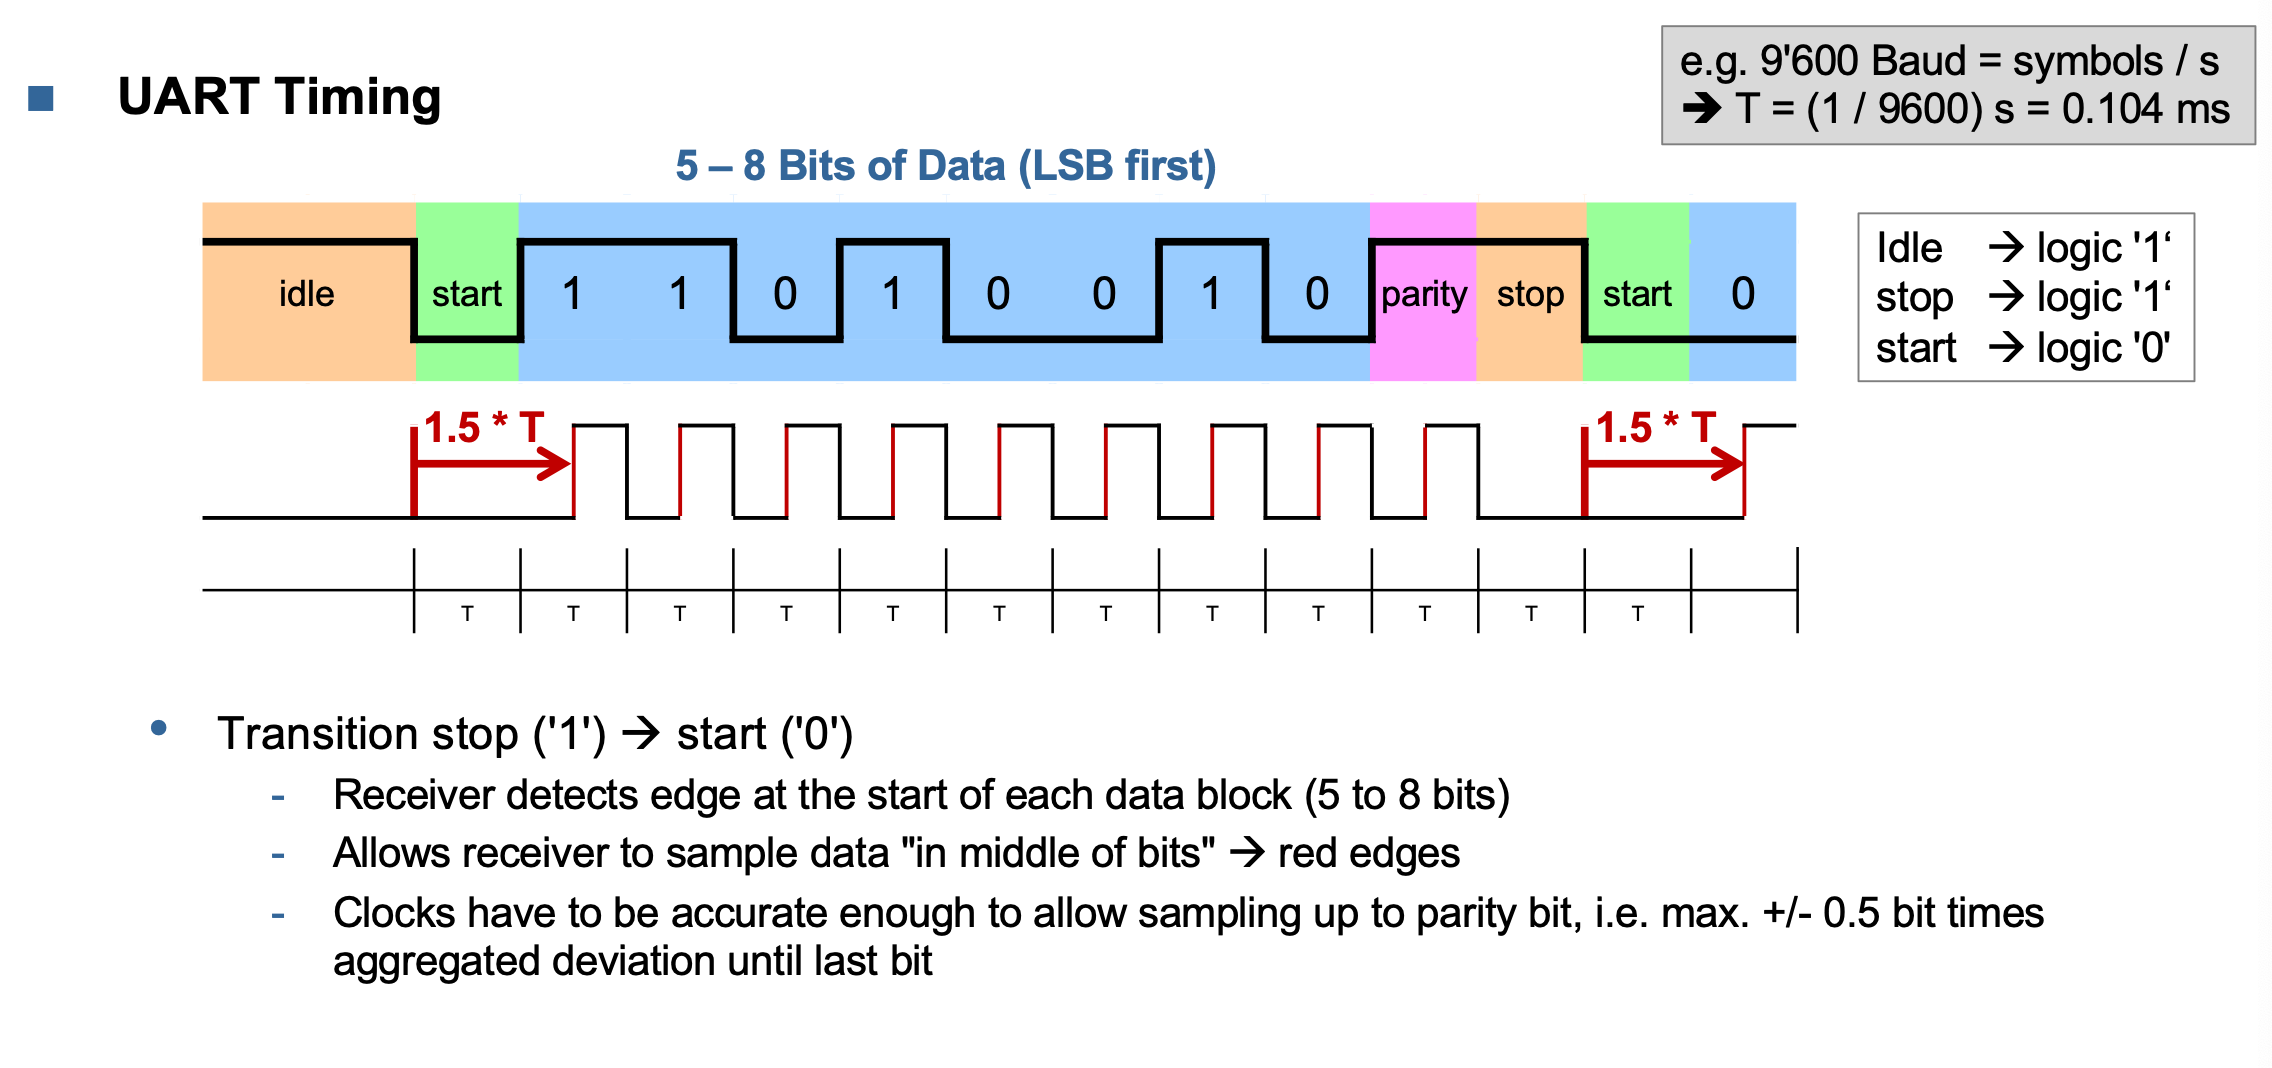
\includegraphics[width=0.3\textwidth]{sections/images/uart_timing.png}

\subsubsection{U(S)ART STM32F4}
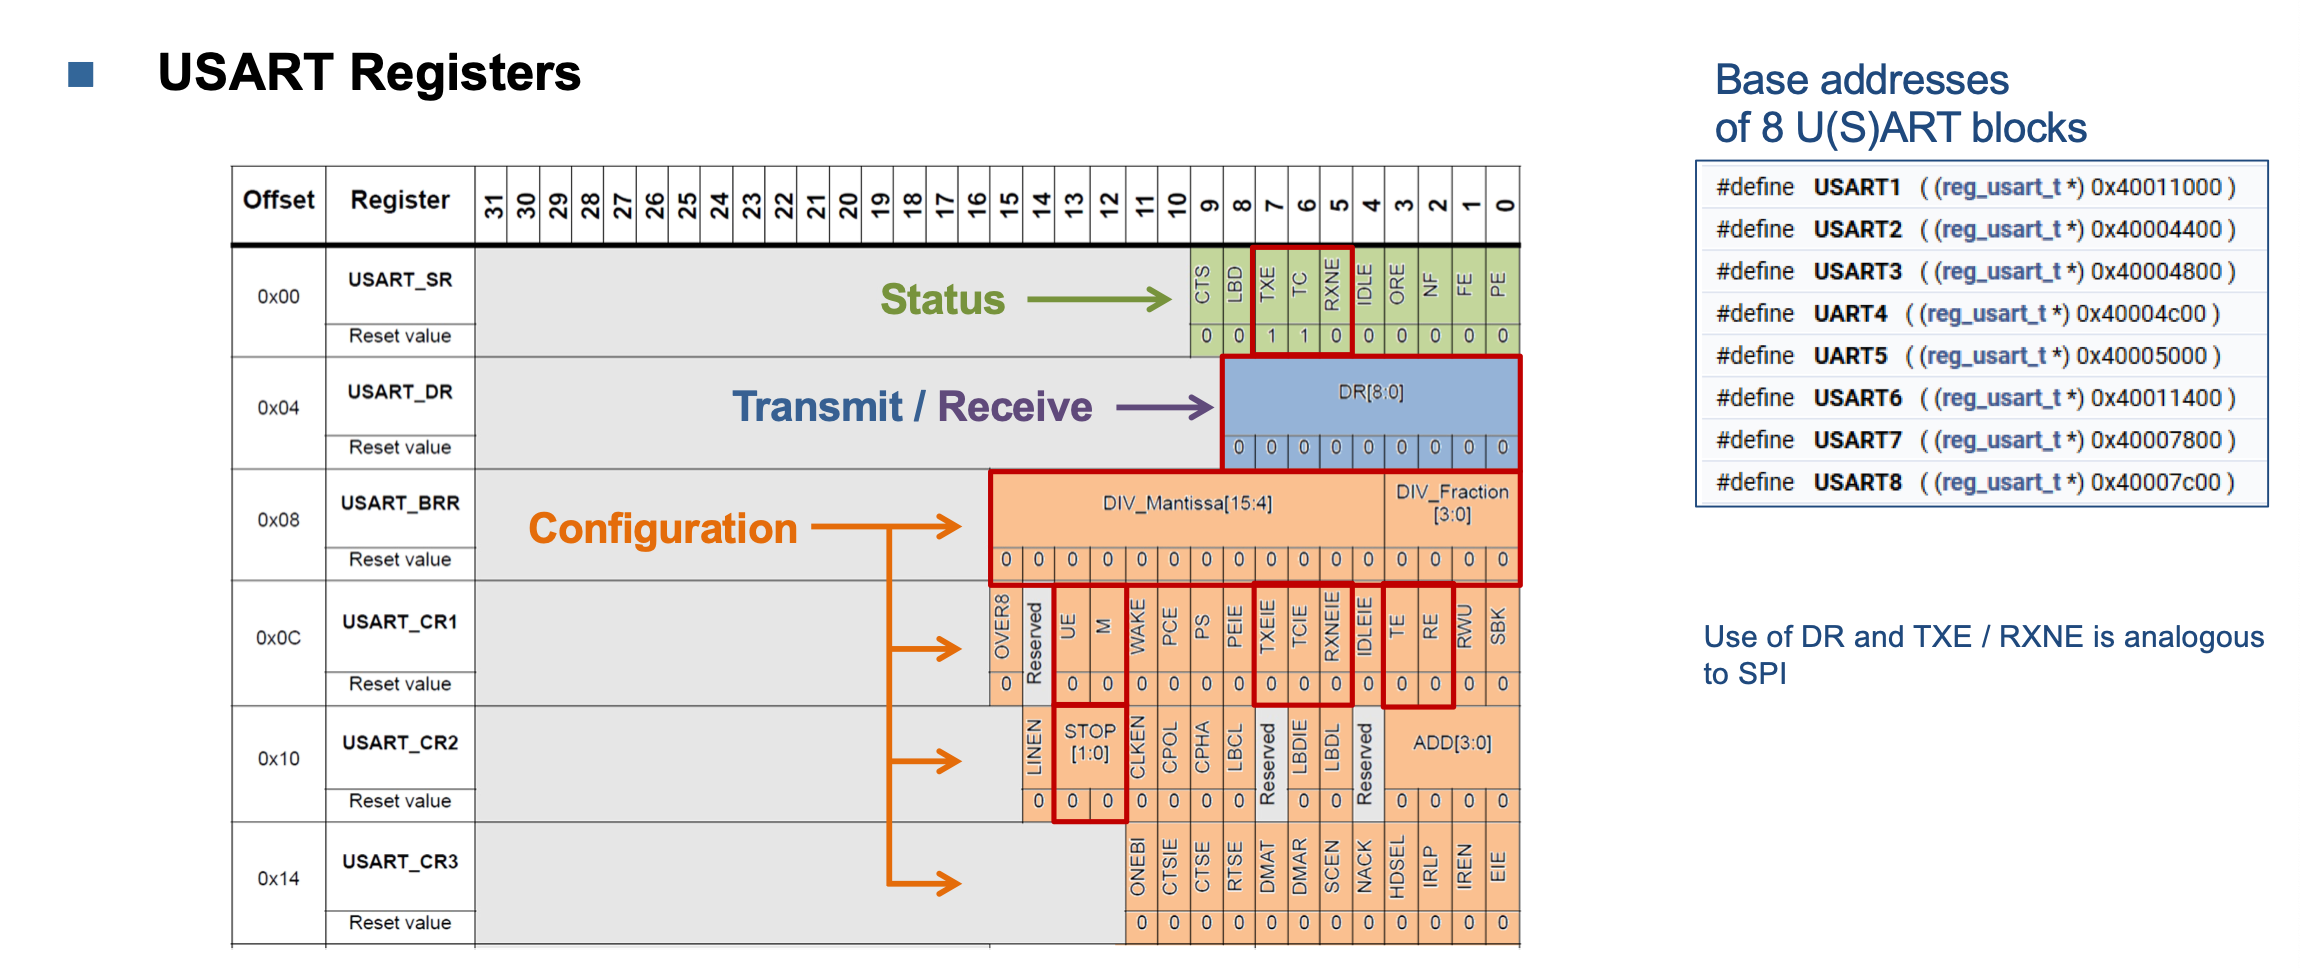
\includegraphics[width=0.3\textwidth]{sections/images/uart_registers.png}

\subsubsection{UART Beispiel}
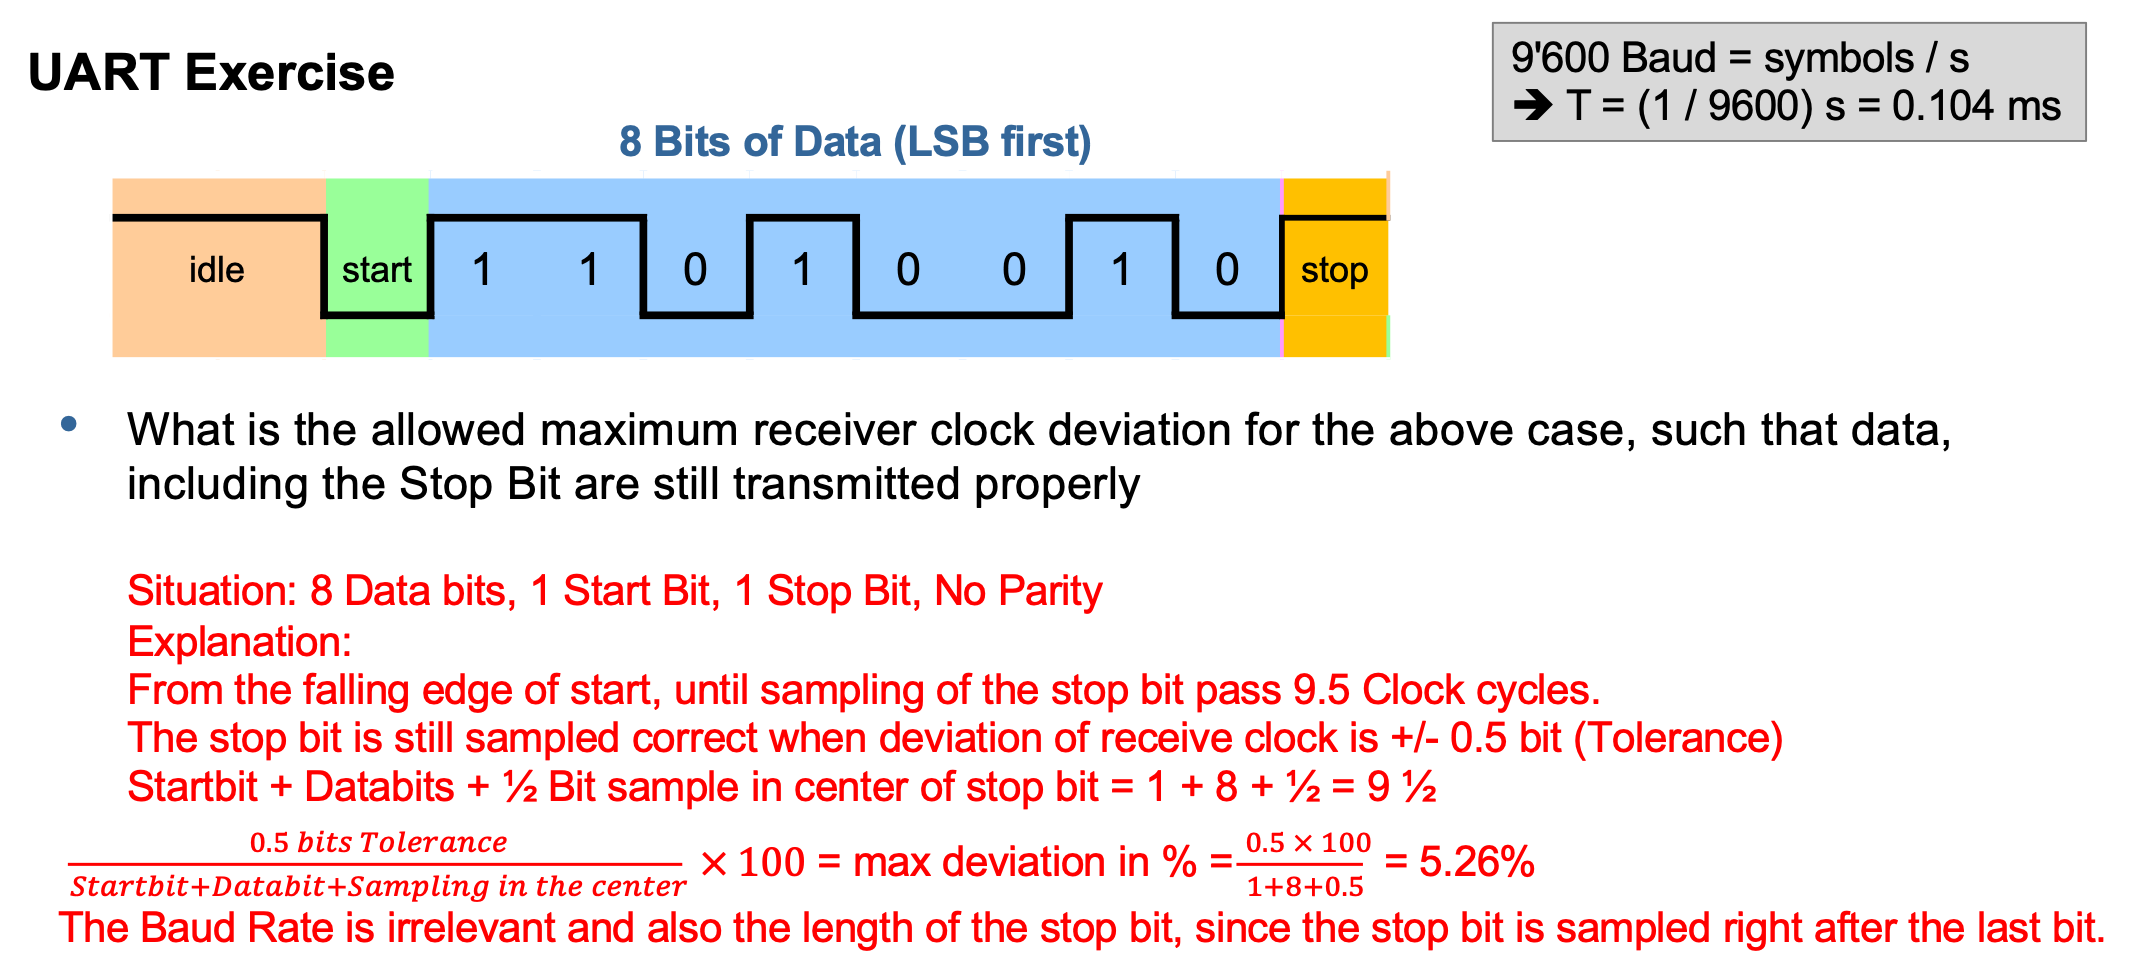
\includegraphics[width=0.3\textwidth]{sections/images/uart_example.png}

\subsection{I2C - Inter-Integrated Circuit}
\begin{itemize}
    \item 2-Draht Bus: Clock (SCL) und Data (SDA)
    \item Synchron, Halbduplex
    \item Jedes Gerät auf dem Bus hat eine eigene Adresse
    \item 8-Bit Datenübertragung
    \item Datenübertragung wird vom Master oder von adressierten Slaves initiiert
    \item Multi-Master Betrieb möglich
    \item Datenänderung nur bei CLK=0
\end{itemize}
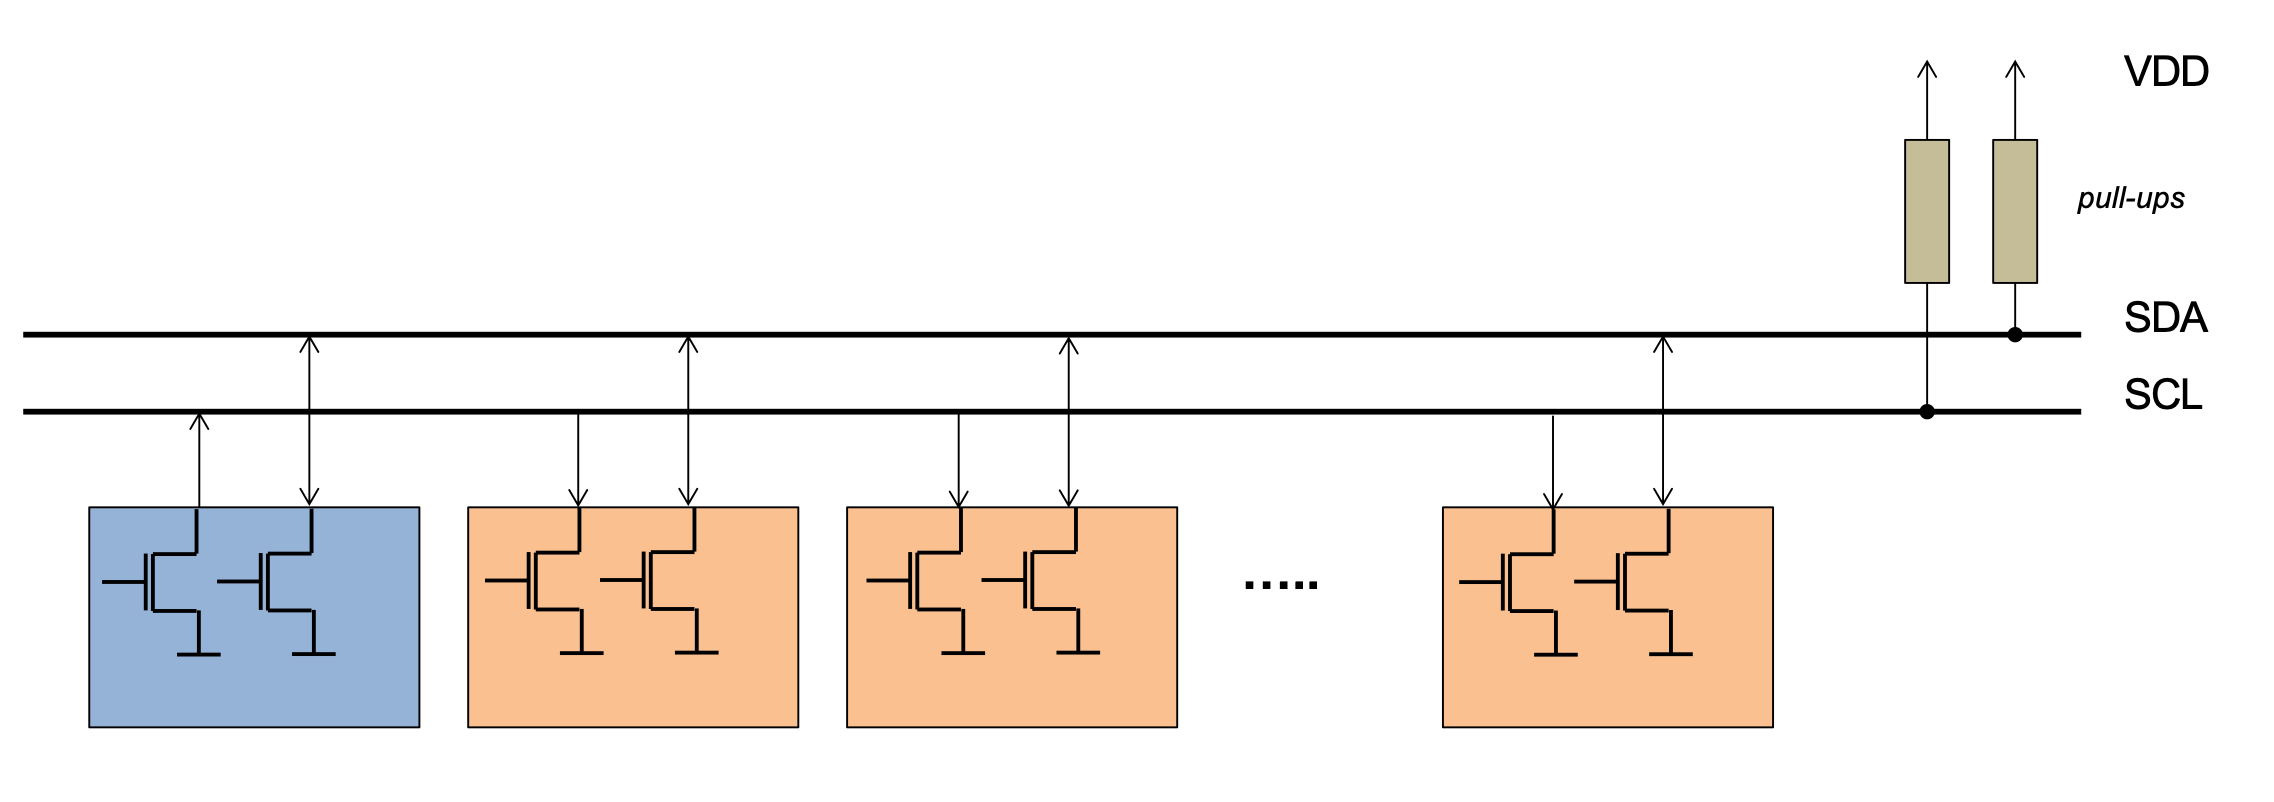
\includegraphics[width=0.3\textwidth]{sections/images/i2c.png}\\
I2C basiert auf open-drain Transistoren.
\subsubsection{I2C Datenübertragung}
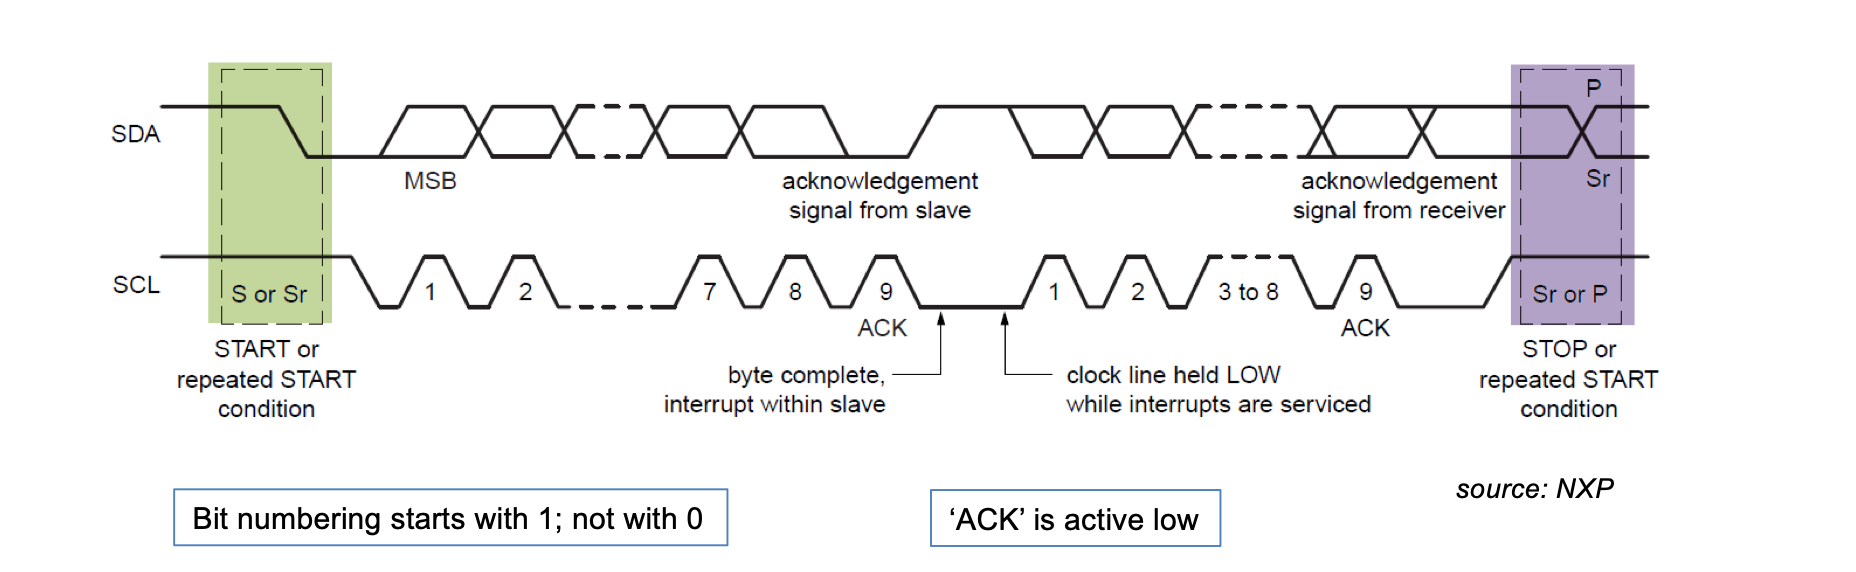
\includegraphics[width=0.3\textwidth]{sections/images/i2c_transfer.png}

\subsubsection{I2C Acknowledge}
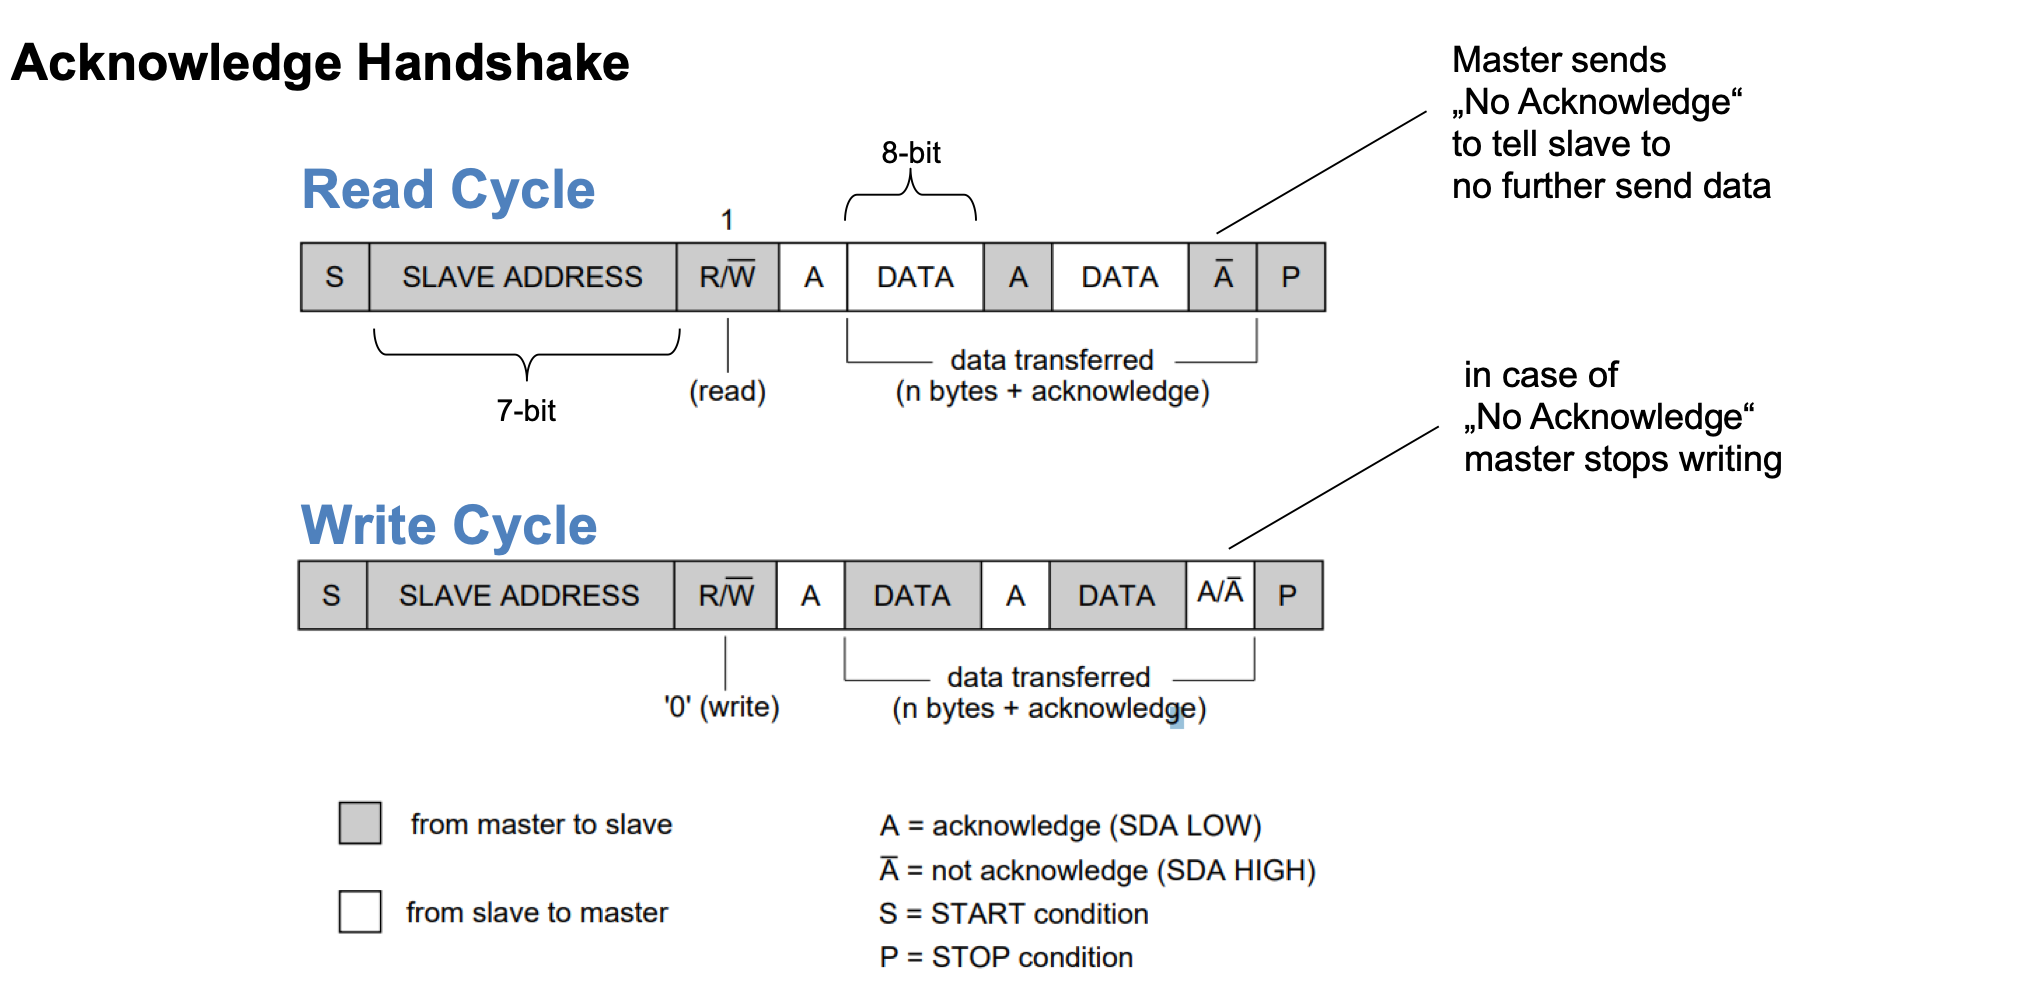
\includegraphics[width=0.3\textwidth]{sections/images/i2c_ack.png}

\subsubsection{I2C Timing-Diagramm}
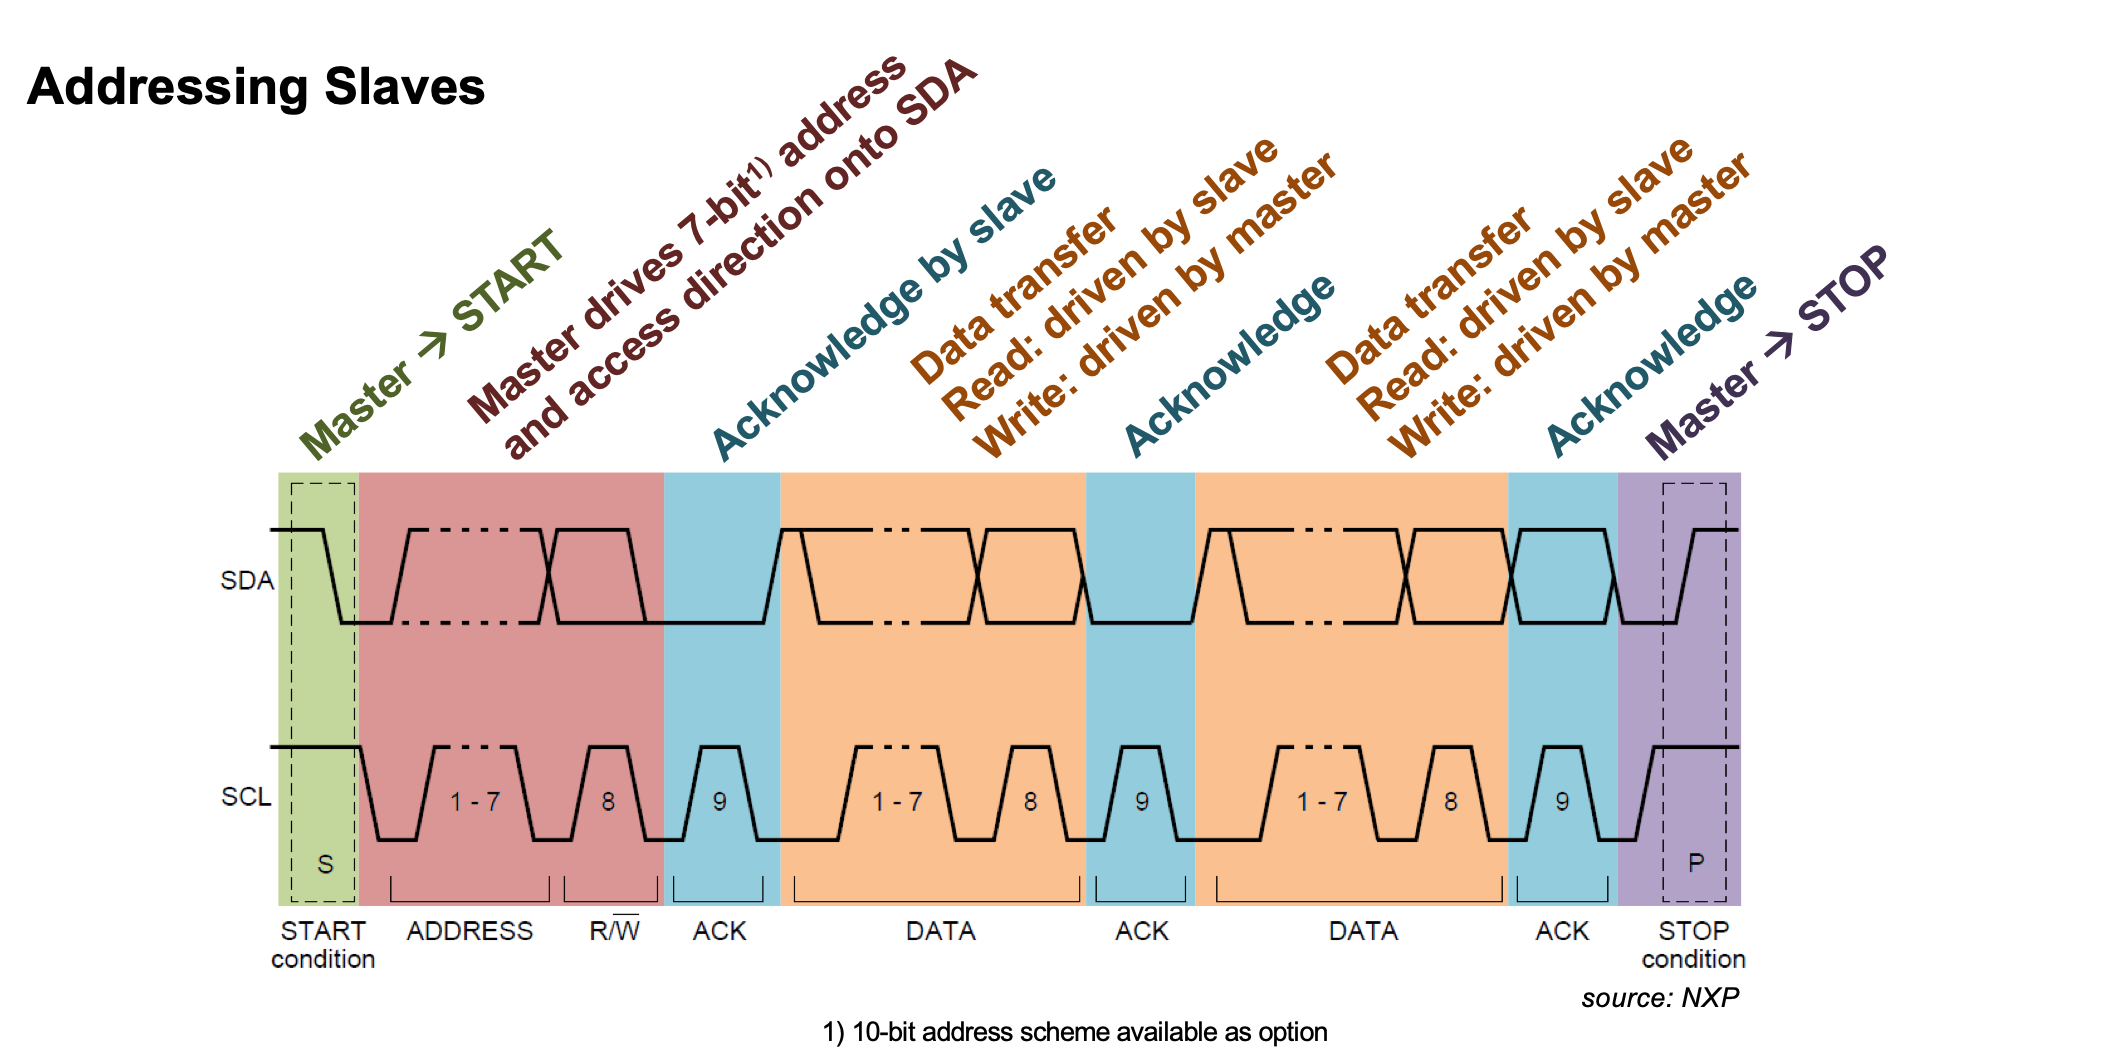
\includegraphics[width=0.3\textwidth]{sections/images/i2c_timing.png}

\subsubsection{I2C Write/Read Zyklus}
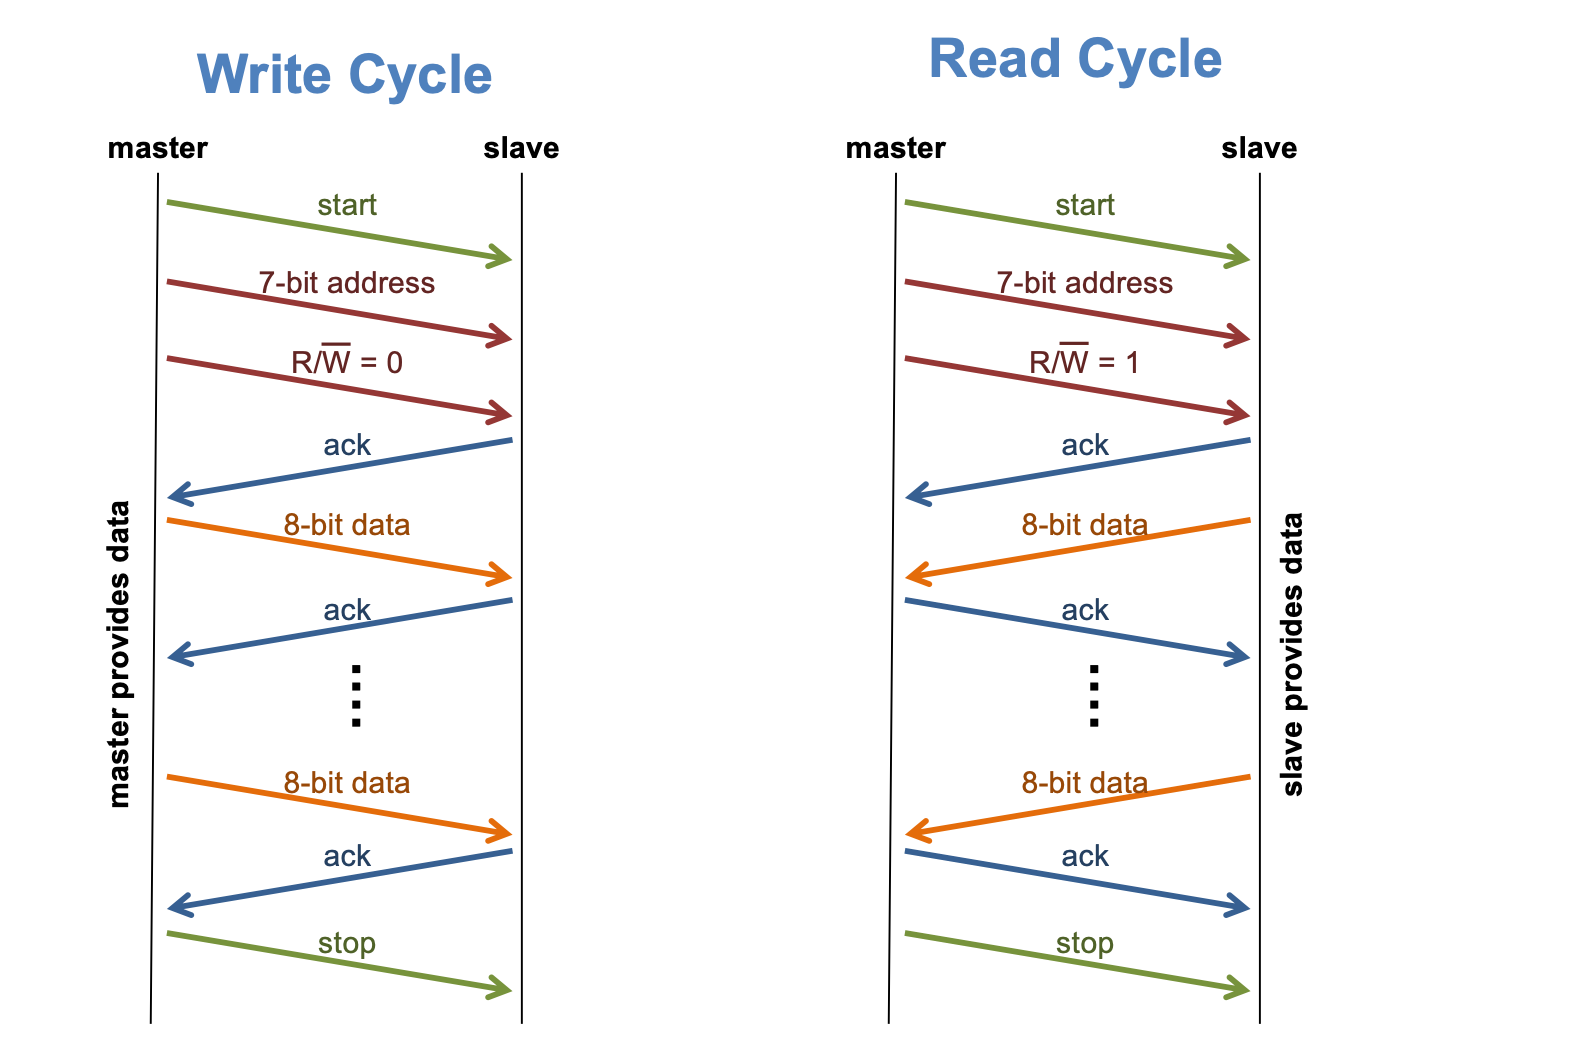
\includegraphics[width=0.3\textwidth]{sections/images/i2c_cycle.png}

\subsubsection{I2C STM32F4}
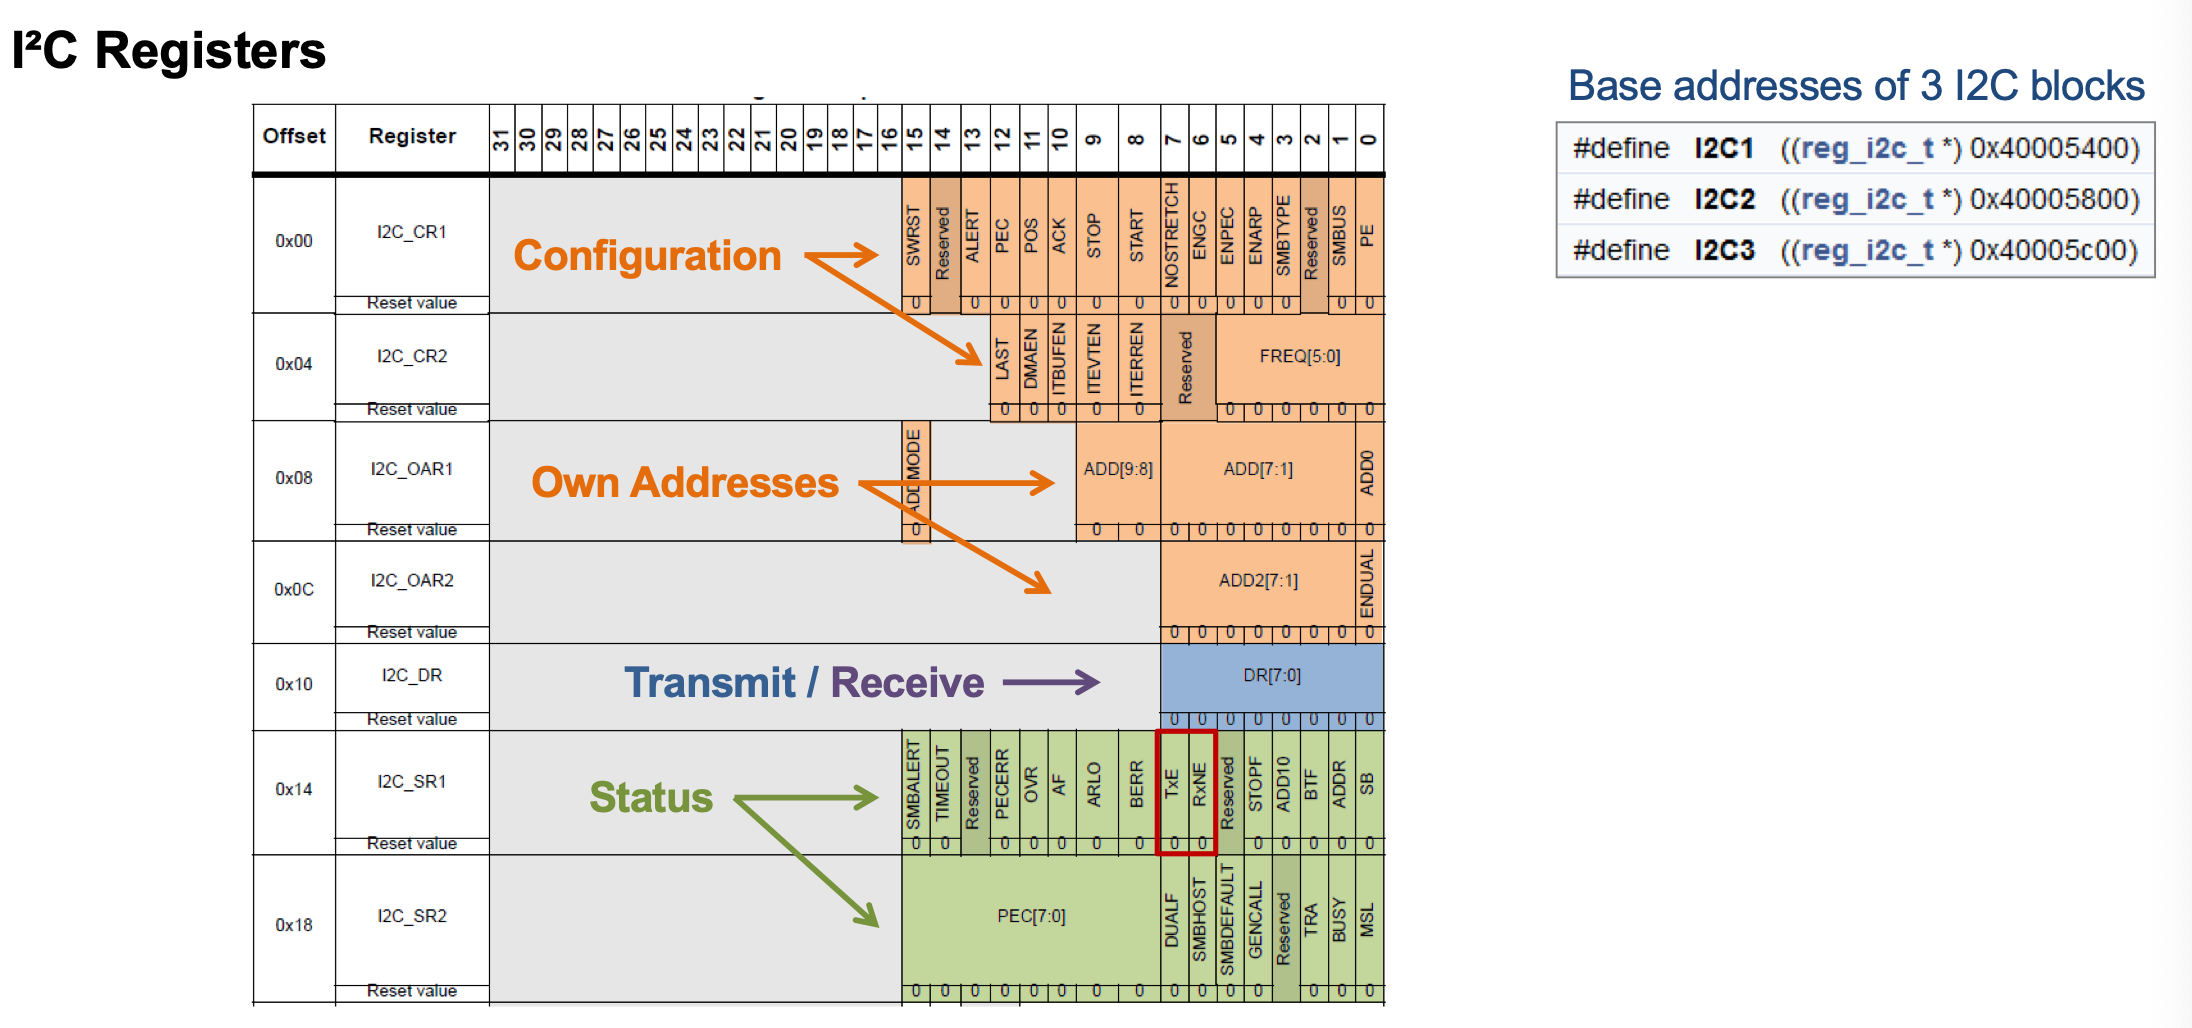
\includegraphics[width=0.3\textwidth]{sections/images/i2c_registers.png}
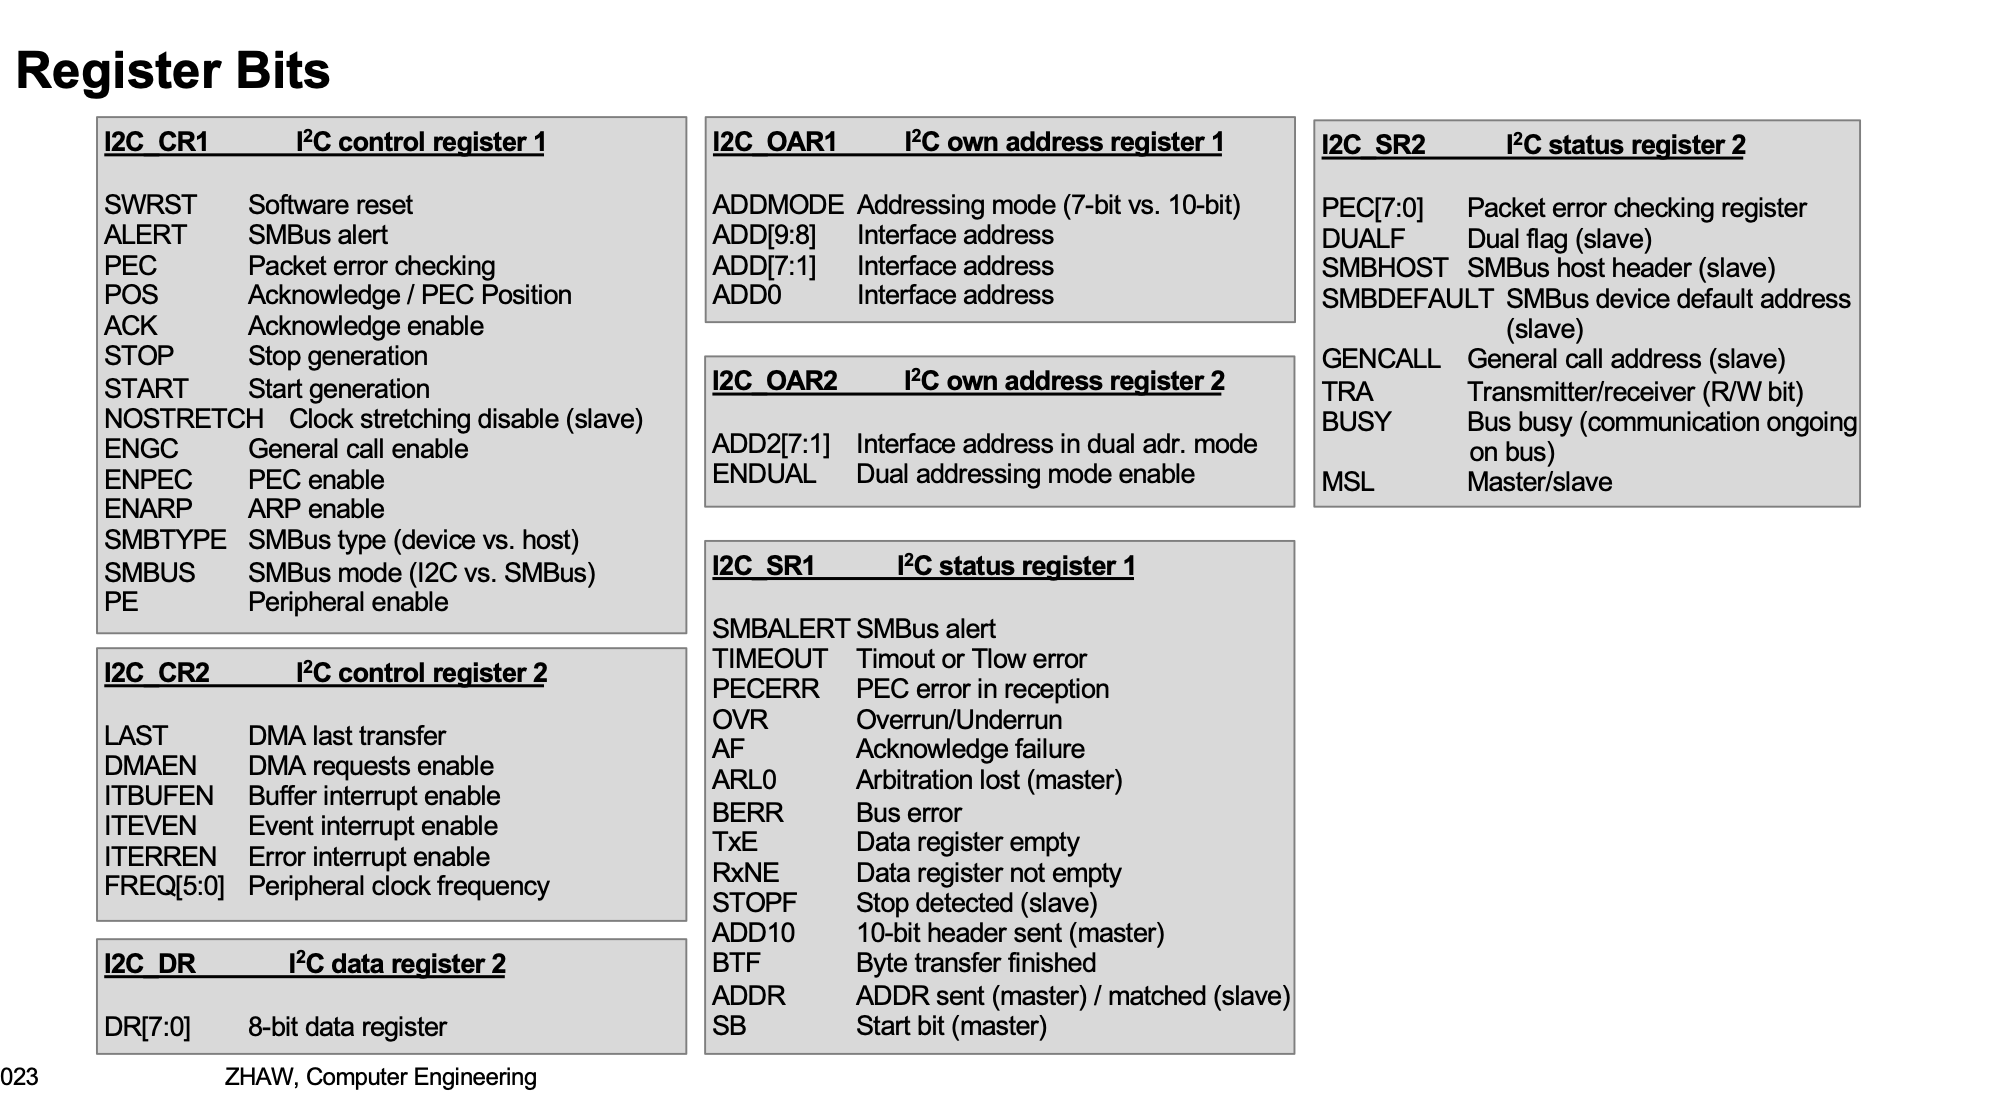
\includegraphics[width=0.3\textwidth]{sections/images/i2c_register_bits.png}

\subsubsection{I2C Beispiel}
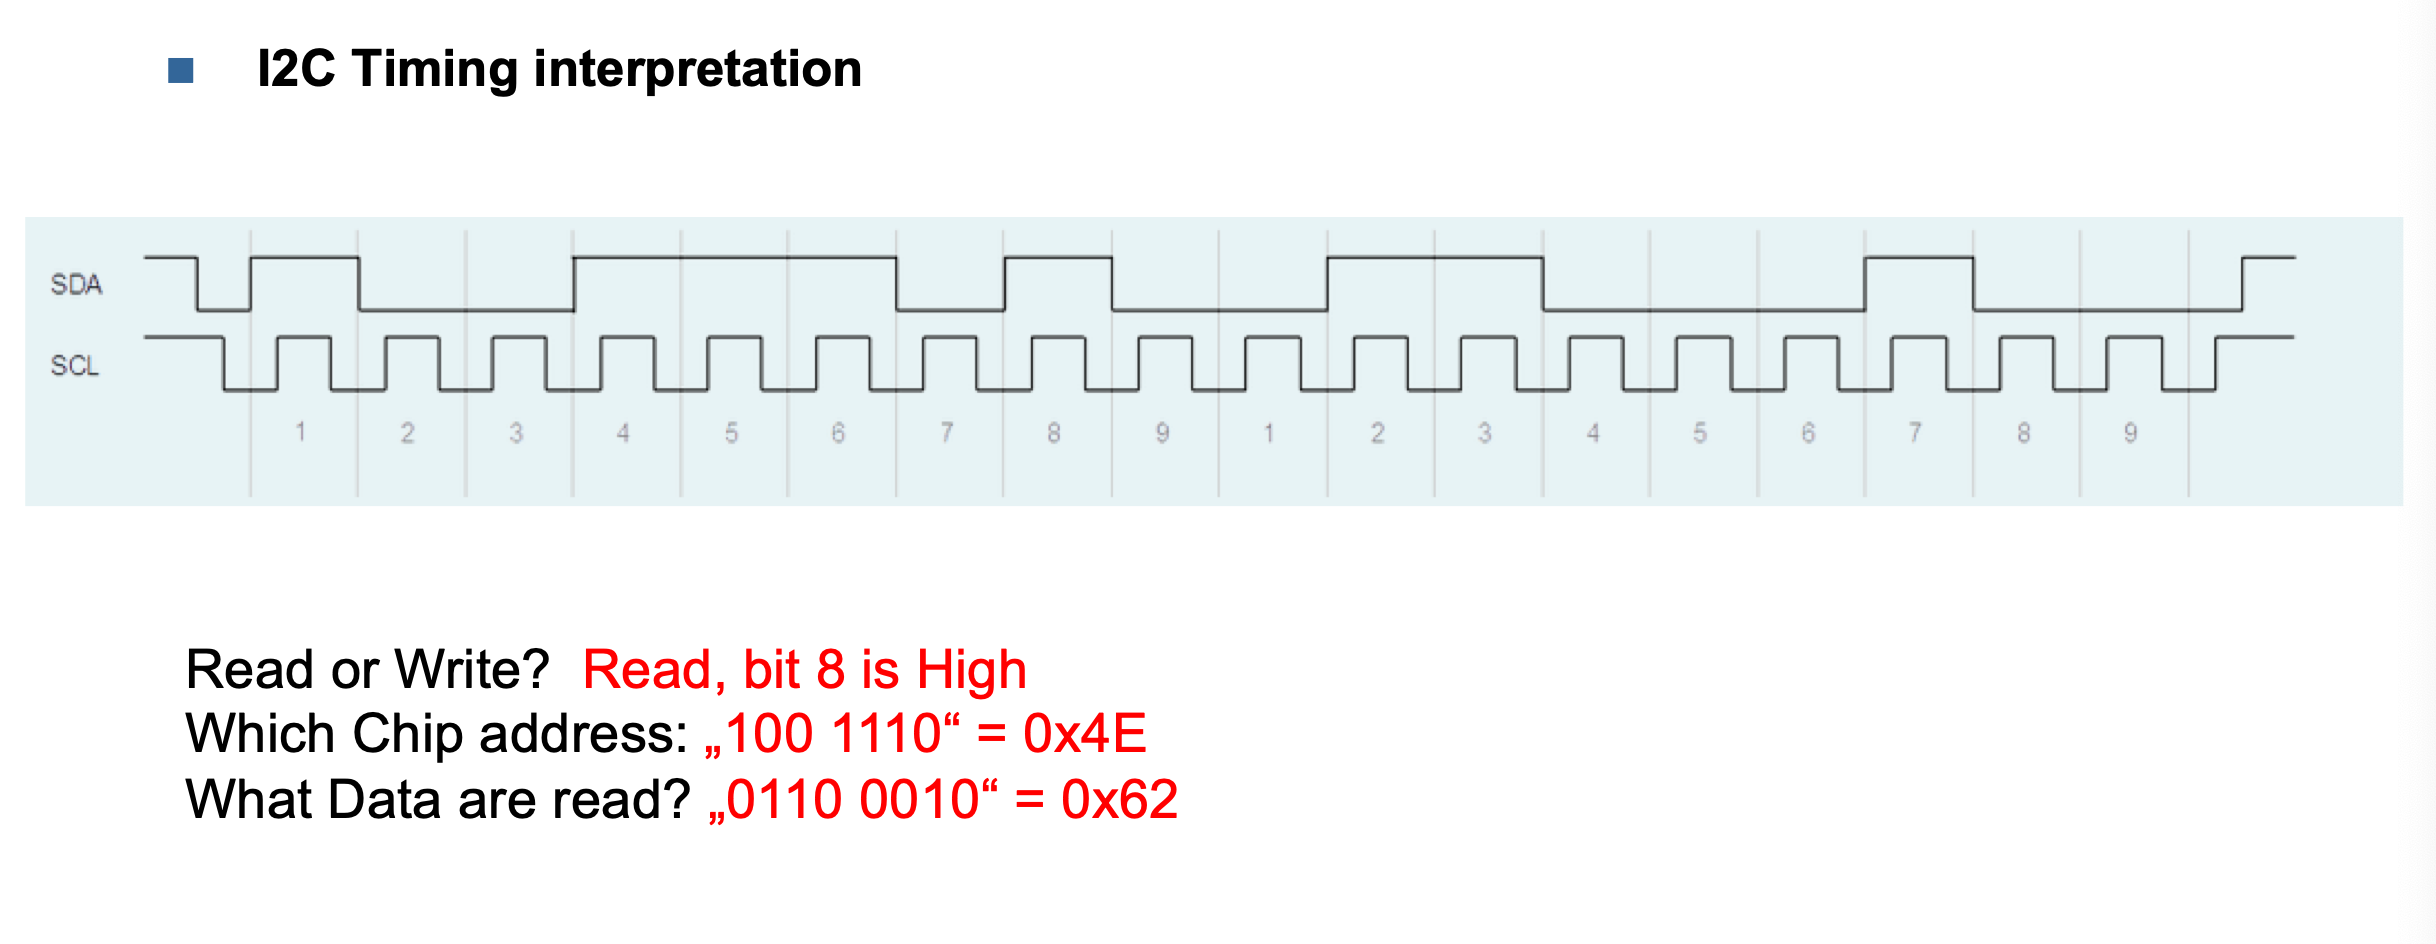
\includegraphics[width=0.3\textwidth]{sections/images/i2c_example.png}